% !TeX root = ../main.tex
% **************************************************************************
\xchapter{应用信息瓶颈理论的鲁棒视觉问答方法}{Correlation Information Bottleneck: Towards Adapting Pretrained Multimodal Models for Robust Visual Question Answering}


受益于大规模视觉语言预训练技术,视觉问答模型在标准数据集上的性能已经达到人类水平。然而,视觉语言预训练模型获得的表征通常不可避免地包含与下游视觉问答任务无关的和冗余的信息,这会导致预训练模型生成的表征统计上的虚假关联,使模型对输入变化的敏感性降低,从而影响其输入鲁棒性。为了在将视觉语言预训练模型迁移至视觉问答任务时提高模型的输入鲁棒性,本章提出了基于相关信息瓶颈理论的方法。整体而言,该方法通过最小化输入与中间表征之间的相互信息同时最大化输出和表征之间的互信息实现表征中信息压缩与冗余之间的平衡。此外,本章为多模态输入和表征之间的互信息估计提供了紧凑的理论上界,通过度量多模态输入和表征之间的多种信息关联有效地指导视觉问答模型学习更鲁棒的表征并促进多模态对齐。在五个鲁棒性相关的数据集上进行的广泛实验表明使用本章提出的相关信息瓶颈理论为训练目标能显著提高视觉问答模型的输入鲁棒性,一定程度上解决了当前视觉问答模型对视觉语言输入变化鲁棒性不足的问题。


% **************************************************************************
\xsection{引言}{Introduction}

视觉问答~\cite{antol2015vqa}是视觉语言领域极具代表性的任务之一。
近来,大规模视觉语言预训练模型~\cite{wang2021simvlm,wang2021vlmo,li2022blip}显著地提高了下游视觉问答任务的性能,使视觉问答模型性能能够达到人的水平。
然而,用有限的数据对极大规模的视觉语言预训练模型进行微调通常会面临过拟合和泛化能力差的问题。
这导致视觉语言预训练模型在提升视觉问答鲁棒性方面的效果相对有限,远不及其对视觉问答准确性的提升。
因此,本章探讨视觉问答模型的输入鲁棒性(Input Robustness)并致力于在为视觉问答任务微调视觉语言预训练模型时,提高模型输入鲁棒性。
输入鲁棒性指的是视觉问答模型应对图像中的视觉变化,如问题相关的目标的移除~\cite{agarwal2020towards}、问题中的语言变化如单词替换和句子改写~\cite{shah2019cycle,whitehead2020learning} 和多模态捷径学习~\cite{dancette2021beyond},的能力。
实际上,在微调过程中,视觉问答任务通常被表述为多答案分类问题或者文本生成问题,其中视觉语言预训练模型充当具有丰富知识的表征提取器。
因此,提高输入鲁棒性本质上就是使获得的表征更加紧凑和更加任务相关。


为了实现这一目标,本章提出从信息理论的角度提高视觉问答模型的输入鲁棒性。
从该角度分析视觉问答模型鲁棒性差可能的原因,本文发现视觉语言预训练模型生成的表征不可避免地包含与下游视觉问答任务无关的和冗余的信息。
然而,不相关的信息会鼓励视觉问答模型学习表征和标签之间统计上的虚假关联,与任务无关的冗余信息会降低视觉问答系统对输入变化的敏感度。
这两种信息都会损害视觉问答模型的鲁棒性。
因此,在为视觉问答任务微调视觉语言预训练模型时,为了获得更鲁棒的表征,本章期望在保留相关信息的同时,丢弃表征中的不相关和冗余信息。信息瓶颈理论(Information Bottleneck,IB)~\cite{tishby2000information}能有效地平衡表征的压缩和冗余。
受此启发,为训练更鲁棒的视觉问答模型,本文利用信息瓶颈原理来寻找所获得表征的最小充分统计量。


具体来说,本章提出了相关信息瓶颈理论(Correlation Information Bottleneck, CIB)在迁移预训练视觉语言模型至下游视觉问答任务时提高模型的输入鲁棒性。
整体而言,CIB通过最小化输入与表征之间的相互信息并最大化输出和表征之间的互信息来寻求表征中信息压缩和冗余之间的平衡,以便促进视觉语言表征收敛到最小充分统计量。
而为了准确估计多模态输入和表征之间的互信息,本章推导多模态输入和表征之间的对称联合互信息紧凑的理论上界。
该上界度量不同模态之间的内部关联,不仅考虑单模态输入和表征之间的关联还考虑了不同模态表征之间的关联,以此来指导视觉问答模型学习更鲁棒的表征和捕获表征间更真实的关系。特别是不同模态表征之间的关联能有效地促进多模态对齐。
此外,考虑到视觉语言预训练模型的结构差异,本章在CIB估计时统一了视觉语言预训练模型的中间表征。

本章的主要贡献概括如下:
\begin{itemize}
\item 提出了相关信息瓶颈理论。在迁移视觉语言预训练模型至视觉问答任务时,该理论通过最小化输入与表征之间的相互信息并最大化输出和表征之间的互信息来平衡表征中的信息压缩和冗余,有效地提高了模型的输入鲁棒性。
\item 为多模态输入和表征之间互信息的估计提供了紧凑的理论上界。该上界通过度量不同模态输入和表征之间的内部关联来指导视觉问答模型学习更鲁棒的表征并促进多模态对齐。
\end{itemize}



% **************************************************************************
\xsection{预备知识}{Preliminary} 

本节首先阐述基于视觉语言预训练模型微调的视觉问答任务设置;然后介绍信息瓶颈理论在表征学习中的应用。

\xsubsection{任务的表述}{Problem Definition}

在微调过程中,单双流视觉语言模型将视觉问答任务表述为多答案分类问题,而编解码视觉语言模型则将其表述为文本生成任务。
给定视觉问答数据集$\mathcal{D}=\{(I, Q, a)\in \mathcal{I}\times \mathcal{Q}\times \mathcal{A} \}$,其中$I$表示图像、$Q$表示问题、$a$是对应的答案,视觉语言预训练模型以图像-问题对作为输入并使用附加的视觉问答分类模块输出答案的概率分布$\Ymat$。
而输入的图像和问题通常会进一步表示为$K$个图像区域集合和$L$个问题token序列。


\xsubsection{从信息瓶颈的角度理解表征学习}{IB View for Representation Learning}

从信息论的角度来看,视觉语言预训练模型学习鲁棒的表征$\Tmat$等效于在保留有关输出$\Ymat$的信息的同时从输入$\Xmat$中移除不相关和冗余的信息。
这是因为对于给定的视觉问答任务,不相关和冗余的信息可能会鼓励视觉语言预训练模型学习答案标签和输入之间虚假的相关。
因此,信息瓶颈原理可以将视觉语言表征学习表述为一种信息理论上的权衡,并通过最大化拉格朗日乘子来学习一个最优表征
\begin{equation}
\begin{aligned} 
\mathcal{L}_{\text{IB}} := I(\Ymat; \Tmat) - \beta I(\Xmat; \Tmat),
\end{aligned}
\label{eq:ib} 
\end{equation}
式中,$\beta \ge 0$控制着压缩与表征之间的平衡;$I(\cdot; \cdot)$表示互信息。


% **************************************************************************
\xsection{相关信息瓶颈理论}{Correlation Information Bottleneck} 

本节首先详细介绍了本章提出的相关信息瓶颈理论;然后阐述了如何将该理论应用于面向鲁棒视觉问答的视觉语言预训练模型微调。

% ********************************************************************
\xsubsection{理论推导}{Derivation of CIB}
\label{sec:CIB}

在视觉语言学习中,给定两种模态的输入$\Xmat^v$和$\Xmat^l$,视觉语言预训练模型在学习对应的中间表征$\Tmat^v$和$\Tmat^l$的同时通过最大化所获得的表征与输出$\Ymat$之间的互信息来保证表征包含充分的用于预测$\Ymat$的信息。
为了将原始的信息瓶颈原理扩展到视觉语言学习中,本章首先将视觉语言输入和对应的中间表征分别组合为$\Xmat=[\Xmat^v, \Xmat^l]$和$\Tmat=[\Tmat^v, \Tmat^l]$;然后通过将公式~(\refeq{eq:ib})中的互信息项展开来推导可微的信息瓶颈估计值。

具体来说,为了在视觉语言学习中推导出可微分的信息瓶颈估计,本文首先考虑$I(\Ymat; \Tmat)$项,它可以利用条件概率的定义重写为以下形式:
\begin{equation}
\begin{aligned}
I(\Ymat; \Tmat) = \int p(\yv, \tv) \log \frac{p(\yv|\tv)}{p(\yv)} \, {d\yv \, d\tv \,}. 
\end{aligned}
\label{eq:mi}
\end{equation} 
因为条件概率$p(\yv|\tv)$难以求解,本文采用BA下界~\cite{agakov2004algorithm}来估计$I(\Ymat; \Tmat)$,具体如下:
\begin{equation}
\begin{aligned}
I(\Ymat; \Tmat) \ge \int p(\yv, \tv) \log q(\yv|\tv) \, {d\yv \, d\tv \,}\, - \int p(\yv) \log p(\yv)\, d\yv, 
\end{aligned}
\label{eq:lower}
\end{equation}
式中,$q(\yv|\tv)$是$p(\yv|\tv)$可计算的辅助分布;标签的熵$H(\Ymat) = - \int p(\yv) \log p(\yv)\, d\yv$独立于优化过程。
因此,忽略$H(\Ymat)$,公式~(\refeq{eq:lower})中剩余项就等于$-H(\Ymat|\Tmat)$。这也意味着最大化$I(\Ymat; \Tmat)$的下界等同于最小化给定任务的损失。


接下来,考虑模型输入和对应的中间表征之间的互信息,即公式~(\refeq{eq:ib})中的$I(\Xmat; \Tmat)$项。
为了准确地估计$I(\Xmat; \Tmat)$,本章将其展开为$I(\Xmat^v, \Xmat^l; \Tmat^v, \Tmat^l)$并为其推导了紧促的理论上界。
因为$I(\Xmat^v, \Xmat^l; \Tmat^v, \Tmat^l)$包含不同的内部关联,如视觉输入和表征间的相关、语言输入和表征间的相关以及视觉语言表征之间的相关。
这些相关不仅会促进模型学习更鲁棒的中间表征还会促进视觉和语言表征的对齐。
因此,本章提出最大化相关信息瓶颈(CIB)公式:
\begin{equation}
\begin{aligned} 
\mathcal{L}_{\text{CIB}} := I(\Ymat; \Tmat) - \beta I(\Xmat^v, \Xmat^l; \Tmat^v, \Tmat^l), 
\end{aligned}
\label{eq:CIB}
\end{equation}
式中,$I(\Xmat^v, \Xmat^l; \Tmat^v, \Tmat^l)$是联合互信息~\cite{bennasar2015feature}的一种对称变体。为了有效地估计$I(\Xmat^v, \Xmat^l; \Tmat^v, \Tmat^l)$,本文首先基于互信息的性质和表征学习中的数据处理不等式~\cite{federici2020learning}将其展开。推导结果可表述为定理~\ref{thm:JMI}(证明见附录A)。

\begin{theorem}[互信息$I(\Xmat^v, \Xmat^l; \Tmat^v, \Tmat^l)$的上界]
\label{thm:JMI}
给定两组随机变量$\Xmat=[\Xmat^v, \Xmat^l]$和$T=[\Tmat^v, \Tmat^l]$,互信息$I(\Xmat^v, \Xmat^l; \Tmat^v, \Tmat^l)$的下界可表述为:
\begin{equation}
\begin{aligned}
I(\Xmat; \Tmat) = I(\Xmat^v, \Xmat^l; \Tmat^v, \Tmat^l) \le \underbrace{I(\Xmat^v; \Tmat^v)}_{\text{\small{\ding{202}}}} + \underbrace{I(\Xmat^l; \Tmat^l)}_{\text{\small{\ding{203}}}} \underbrace{- I(\Tmat^v; \Tmat^l)}_{\text{\small{\ding{204}}}} + \underbrace{\SKL}_{\text{\small{\ding{205}}}}, 
\end{aligned}
\label{eq:c4_JMI}
\end{equation}
式中,$\SKL$表示对称KL散度,可以通过平均两个KL散度$\KL(p(\tv^v|\xv^v)||p(\tv^l|\xv^l))$和$\KL(p(\tv^l|\xv^l)||p(\tv^v|\xv^v))$来计算。
\end{theorem}

在获得$I(\Xmat^v, \Xmat^l; \Tmat^v, \Tmat^l)$的估计后,$\mathcal{L}_{\text{CIB}}$可以表述为定理~\ref{thm:CIB}。

\begin{theorem}(相关信息瓶颈$\mathcal{L}_{\text{CIB}}$的下界) 
给定两组随机变量$\Xmat = [\Xmat^v, \Xmat^l]$,两个确定性函数$f_{\theta^v}$和$f_{\theta^l}$使得$\Tmat^v = [\Tmat^v_{1}, \Tmat^v_{2}, ..., \Tmat^v_{K}] = [f_{\theta^v}(\Xmat^v_{1}), f_{\theta^v}(\Xmat^v_{2}), ..., f_{\theta^v}(\Xmat^v_{K})]$ 和 $\Tmat^l = [\Tmat^l_{1}, \Tmat^l_{2}, ..., \Tmat^l_{L}]$ $= [f_{\theta^l}(\Xmat^l_{1}), f_{\theta^l}(\Xmat^l_{2}), ..., f_{\theta^l}(\Xmat^l_{L})]$。
则,相关信息瓶颈CIB的下界可表述为
\begin{equation} 
\begin{aligned}
\mathcal{L}_{\text{CIB}} &= I(\Ymat; \Tmat) - \beta I(\Xmat^v, \Xmat^l; \Tmat^v, \Tmat^l)\\ 
&\ge I(\Ymat; \Tmat) - \beta\left[I(\Xmat^v; \Tmat^v) + I(\Xmat^l; \Tmat^l) - I(\Tmat^v; \Tmat^l) + \SKL \right]. 
\end{aligned}
\label{eq:CIB_all}
\end{equation} 
\label{thm:CIB}
\end{theorem} 

定理~\ref{thm:CIB}表明在视觉语言表征学习时,若将互信息$I(\Ymat; \Tmat)$视为任务相关的训练目标,那么$-\beta I(\Xmat^v, \Xmat^l; \Tmat^v, \Tmat^l)$则可被视为用来约束表征的紧凑性的互信息正则项。


% ********************************************************************
\xsubsection{CIB在视觉语言预训练模型微调中的应用}{Adapting Pretrained VLMs to VQA with CIB}

如图~\ref{fig:c4_cib_1}、图~\ref{fig:c4_cib_2}和图~\ref{fig:c4_cib_3} 所示,视觉语言预训练模型具有三种典型的Transformer结构(单流、双流和编解码结构)。
在为视觉问答任务微调视觉语言预训练模型时,为了将这三种典型的结构统一为一种表述,如图~\ref{fig:c4_cib_overall} 所示,本章使用视觉嵌入层($f_{\theta^v}$表示参数化的嵌入层)之后输出的区域级特征或分块特征作为中间视觉表征$\Tmat^v$。
类似地,使用语言嵌入层($f_{\theta^l}$)之后输出的分词级特征作为中间语言表征$\Tmat^l$。
Transformer接下来的所有层($f_{\theta^{{\text{Tran}}}}$)和单双流模型的视觉问答分类器($f_{\theta^\text{H}}$)或编解码模型的解码器($f_{\theta^\text{Dec}}$)一起担任参数化的估计器($f_{\thetav^\text{ans}}$),利用$\Tmat=[\Tmat^v, \Tmat^l]$生成$\Ymat$。
综上,为了使用CIB微调视觉语言预训练模型,本文将公式~(\ref{eq:CIB_all})中的$I(\Ymat; \Tmat)$视为任务相关的损失,即用于答案分类的交叉熵损失,公式~(\ref{eq:CIB_all})中其它项则可视为正则器。

% ********************************************************************
\begin{figure}[!t]
\begin{subfigure}[b]{0.29\textwidth}
\centering
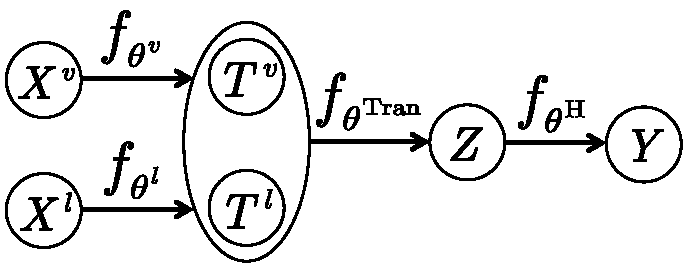
\includegraphics[width=1.0\linewidth]{figure/c4_trans_1.pdf}
\subcaption{单流结构}
\label{fig:c4_cib_1}
\end{subfigure}
\begin{subfigure}[b]{0.37\textwidth}
\centering
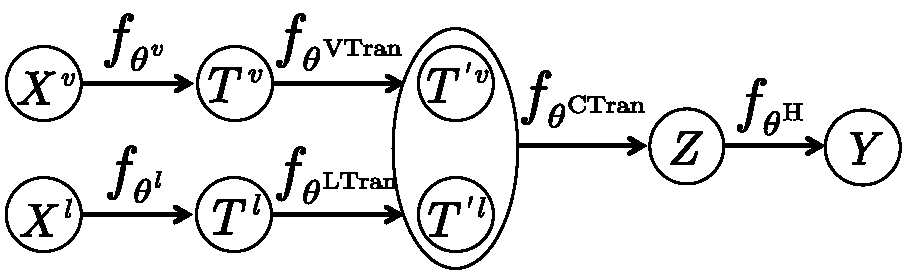
\includegraphics[width=1.0\linewidth]{figure/c4_trans_2.pdf}
\subcaption{双流结构}
\label{fig:c4_cib_2}
\end{subfigure}
\begin{subfigure}[b]{0.29\textwidth}
\centering
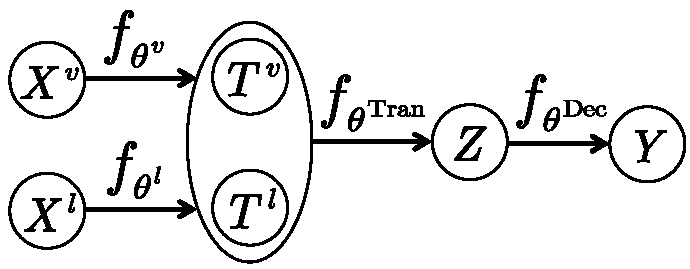
\includegraphics[width=1.0\linewidth]{figure/c4_trans_3.pdf}
\subcaption{编解码结构}
\label{fig:c4_cib_3}
\end{subfigure}
\caption{典型视觉语言预训练模型中信息流图
}
\label{fig:c4_cib}
\end{figure}
% ********************************************************************


\subsubsection{估计CIB中的互信息项}

如定理~\ref{thm:CIB} 所述,除了任务目标相关的项$I(\Ymat; \Tmat)$之外,$I(\Xmat^v, \Xmat^l; \Tmat^v, \Tmat^v\l)$可以被展开为四个可计算的互信息项。
首先,本章考虑单一视觉(语言)模态的输入和表征之间的互信息项。
$\Xmat^v$和$\Xmat^l$本质上是两个随机变量,可以表述为$\Xmat^v = [\Xmat^v_{1}, \Xmat^v_{2}, ..., \Xmat^v_{K}]$和$\Xmat^l = [\Xmat^l_{1}, \Xmat^l_{2}, ..., \Xmat^l_{L}]$。
函数$f_{\theta^v}$和$f_{\theta^l}$将它们映射到表征空间,得到$\Tmat^v = [\Tmat^v_{1}, \Tmat^v_{2}, ..., \Tmat^v_{K}] = [f_{\theta^v}(\Xmat^v_{1}), f_{\theta^v}(\Xmat^v_{2}), ..., f_{\theta^v}(\Xmat^v_{K})]$ 和 $\Tmat^l = [\Tmat^l_{1}, \Tmat^l_{2}, ..., \Tmat^l_{L}] = [f_{\theta^l}(\Xmat^l_{1}), f_{\theta^l}(\Xmat^l_{2}),$ $..., f_{\theta^l}(\Xmat^l_{L})]$。
而对于样本对$\{(\Xmat_i^v, \Tmat_i^v)\}_{i=1}^{K}$ 和 $\{(\Xmat_i^l, \Tmat_i^l)\}_{i=1}^{L}$,在微调过程中条件概率分布$p(\tv^v|\xv^v)$ 和 $p(\tv^l|\xv^l)$是已知的。
因此,本章使用基于采样的可微互信息估计器CLUB~\cite{cheng2020club}来逼近视觉语言输入和表征之间互信息的上界,即
\begin{align}
&\hat{I}(\Xmat^v; \Tmat^v) = \frac{1}{K^2} \sum_{i=1}^{K}\sum_{j=1}^{K} \Big[\log p(\tv_i^v|\xv_i^v) - \log p(\tv_j^v|\xv_i^v)\Big], \\ 
&\hat{I}(\Xmat^l; \Tmat^l) = \frac{1}{L^2} \sum_{i=1}^{L}\sum_{j=1}^{L} \Big[\log p(\tv_i^l|\xv_i^l) - \log p(\tv_j^l|\xv_i^l)\Big]. 
\label{eq:IB_sum_term}
\end{align} 
因为$\Tmat^v \in \mathbb{R}^{K\times d}$ 和 $\Tmat^l\in \mathbb{R}^{L\times d}$的序列长度不同,所以$I(\Tmat^v; \Tmat^l)$很难直接计算。
于是,本章首先使用一个一层的全连接网络将$\Tmat^v$和$\Tmat^l$变换为全局的视觉语言表征$\bar{\Tmat}^v \in \mathbb{R}^{d}$ 和 $\bar{\Tmat}^l\in \mathbb{R}^{d}$。
然后,为了确保公式~(\ref{eq:CIB_all})中的不等式成立,本章应该估计$I(\Tmat^v; \Tmat^l)$的下界。
因此,本章使用NWJ~\cite{poole2019variational}估计$I(\Tmat^v; \Tmat^l)$下界,即
\begin{equation} 
\begin{aligned} 
\hat{I}(\bar{\Tmat}^v; \bar{\Tmat}^l) = \mathbb{E}_{p(\bar{\tv}^v, \bar{\tv}^l)}\left[\log f_{\theta^{\text{FC}}}(\bar{\tv}^v, \bar{\tv}^l)\right] - \frac{1}{e}\mathbb{E}_{p(\bar{\tv}^v) p(\bar{\tv}^l)} \left[f_{\theta^{\text{FC}}}(\bar{\tv}^v, \bar{\tv}^l)\right],
\label{eq:IB_sum_term_rep}
\end{aligned} 
\end{equation} 
式中,$f_{\theta^{\text{FC}}}$是由一个两层的全连接网络实现的确定函数。
最后,因为$p(\tv^l|\xv^l)$ 和 $p(\tv^v|\xv^v)$具有已知的概率密度,可以直接计算对称的KL散度$\SKL$,即
\begin{align} 
&\SKL = \frac{1}{2} \left[\KL\left(p(\tv^v|\xv^v)||p(\tv^l|\xv^l)\right) + \KL\left(p(\tv^l|\xv^l)||p(\tv^v|\xv^v)\right)\right]. 
\label{eq:dskl}
\end{align} 
至此,相关信息瓶颈$\mathcal{L}_{\text{CIB}}$中的所有项均已可计算。


% ********************************************************************
\begin{figure}[!t]
\centering
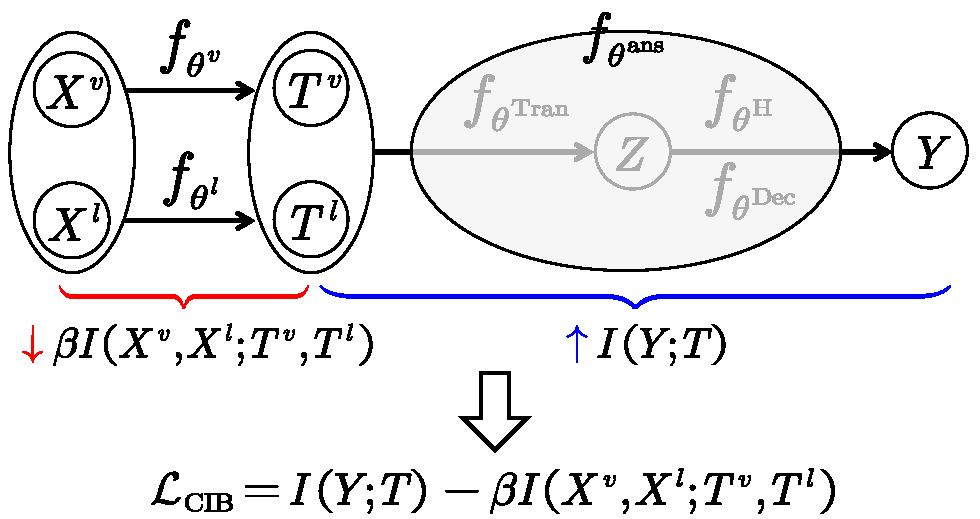
\includegraphics[width=0.5\linewidth]{figure/c4_cib.pdf}
\caption{CIB的示意图}
\label{fig:c4_cib_overall}
\end{figure}
% ********************************************************************



% **************************************************************************
\xsection{实验及结果分析}{Experiment and Result Analysis}


% **************************************************************************
\xsubsection{实验设置}{Experimental Setting}


\subsubsection{数据集}
本章在标准的VQA v2训练集上~\cite{goyal2017making} 微调预训练模型,在VQA-Rep~\cite{shah2019cycle}、VQA P2~\cite{whitehead2020learning}、 IV-VQA~\cite{agarwal2020towards}、 CV-VQA~\cite{agarwal2020towards} 和 VQA-CE~\cite{dancette2021beyond} 上测试输入鲁棒性。
其中,VQA-Rep 和 VQA P2评估视觉问答模型对输入中的语言变化的鲁棒性。
IV-VQA 和 CV-VQA评估视觉问答模型对输入中的视觉变化的鲁棒性。
VQA-CE评估视觉问答模型应对输入中捷径学习的能力。
由于这些输入鲁棒性的评测数据集都是使用VQA v2的验证集创建的,因此本章仅在VQA v2的训练集上使用CIB微调基线模型。

实验数据的统计信息如表~\ref{tab:c4_benchmark}所示。具体来说,VQA-Rep从VQA v2的验证集中采样了40,504个问题,并平均为每个问题收集了3个改写(Rephrasing),最终得到了约162K问题。
VQA P2从VQA v2的验证集中采样了25,814个问题,并为其创建了三种类型的语言变化,即,Paraphrastic (Par)、 Synonymous (Syn)和 Antonymous (Ant),最终获得了约52K个问题。
IV-VQA通过使用基于GAN的生成技术移除图像中与问题无关的物体的方式创建,也就是说改变图像内容并不会改变问题的答案。
与之相反,CV-VQA仅考虑计数类(Num)的问题并移除与问题相关的物体使得对应的答案也应该减一。最终,IV-VQA 和 CV-VQA分别获得了约120k 和 4k的样本。
VQA-CE使用在VQA v2训练集上检测到的shortcuts获得验证集上63,298个反事实样本(Counterexample)和147,681个简单样本(Easy)。


\begin{table}[!t]
\caption{
数据集的统计信息 
% Metric表示数据集提供的输入鲁棒性的评价指标,QType表示问题的类型,len(Q)表示问题的平均长度。
% \#IQ、\#Pert/CE 和 \#Ori/Easy分别表示图像-问题对的总数、添加了输入变化后样本的数量和原始样本数量。
}
\label{tab:c4_benchmark}
\setlength{\tabcolsep}{1.18mm}{
\begin{tabularx}{\textwidth}{@{}lccccccccc}
\toprule

\multirow{2}{*}{Dataset} 
&\multirow{2}{*}{Perturbation} 
&\multirow{2}{*}{Metric}
&\multirow{2}{*}{QType} 
&Training%\multicolumn{1}{c}{\multirow{2}{*}{\makecell{Training\\Dataset}}}
&\multicolumn{4}{c}{Evaluation} 
\\ 
\cmidrule(l){6-9}
& & &
&Dataset
&len(Q) &\#IQ &\#PER/CE &\#ORI/Easy 
\\ 
\midrule
% 换个说法说 
VQA-Rep~\cite{shah2019cycle} 
&Rephrasing 
&CS($m$) 
&All 
&VQA v2 train
&7.15 
&\eqmakebox[log][r]{162k} 
&\eqmakebox[log][r]{121,516} 
&\eqmakebox[log][r]{40,504} 
\\ 
% 改写 
VQA P2~\cite{whitehead2020learning} 
&Par\&Syn\&Ant 
&CS($m$) 
&All 
&VQA v2 train
&6.32 
&\eqmakebox[log][r]{52k} 
&\eqmakebox[log][r]{26,512} 
&\eqmakebox[log][r]{25,814}
\\ 

IV-VQA~\cite{agarwal2020towards} 
&Invariant object 
&\#flips 
&All 
&VQA v2 train
&5.85 
&\eqmakebox[log][r]{120k} 
&\eqmakebox[log][r]{83,700} 
&\eqmakebox[log][r]{36,181} 
\\ 

CV-VQA~\cite{agarwal2020towards} 
&Covariant object 
&\#flips 
&Num  
&VQA v2 train
&5.83 
&\eqmakebox[log][r]{4k} 
&\eqmakebox[log][r]{4,141} 
&\eqmakebox[log][r]{2,641}
\\ 

VQA-CE~\cite{dancette2021beyond} 
&Counterexample 
&- 
&All 
&VQA v2 train
&6.19 
&\eqmakebox[log][r]{214k} 
&\eqmakebox[log][r]{63,298} 
&\eqmakebox[log][r]{147,681}
\\ 
\bottomrule
\end{tabularx}
}
\end{table}



\subsubsection{评价指标}
除了标准的视觉问答性能指标,VQA-Score(见第四章),本章还使用Shah 等人~\cite{shah2019cycle}提出的一致性得分(Consensus Score,CS($m$))来评价视觉问答模型对输入语言变化的鲁棒性。
具体来说,CS($m$)表示所有问题均被正确回答的问题子集的数量与大小为$m$的子集的总数之比。
对每个由一个原始问题和对应的$n$ 个改写组成的问题组$Q$,所有大小为$m$的子集数为$^{n}C_{m}$,则CS($m$)的定义如下:
\begin{equation}
\begin{aligned}
\mathrm{CS}(m) = \sum_{q\in Q^{'}, Q^{'} \subset Q, |Q^{'}|=m} \frac{\InF_{Q^{'}}(q)}{^{n}C_{m}},  
\end{aligned}
\end{equation}
式中,$\InF$是定义在$Q^{'}$上的指示函数,$\InF_{Q^{'}}(q)$表示问题$q$回答正确的集合。
显然,在$m$值越高的情况下,CS($m$)越高,模型就越输入鲁棒。
另外,由于基线视觉语言预训练模型使用了部分数据集的原始样本,这将导致原始样本上的VQA-Score不可靠,因此本章仅测试添加了扰动的样本(PER)和反事实样本(CE)的标准性能。
此外,本章还采用\#flips \cite{agarwal2020towards}评价模型对输入视觉变化的鲁棒性。
\#flips表示视觉内容编辑前后,预测的答案前后不一致的数量占总数的比率。


\subsubsection{基线视觉语言预训练模型}
在本章的实验中,本章使用了三种典型结构的基线视觉语言预训练模型:单流结构(VisualBERT~\cite{li2019visualbert}、VL-BERT$_{\text{B}}$~\cite{su2019vl} 和 UNITER$_{\text{B}}$~\cite{chen2020uniter})、双流结构(LXMERT~\cite{tan2019lxmert} 和 ViLBERT~\cite{lu2019vilbert})和编解码结构(VL-T5~\cite{cho2021unifying} 和 ALBEF~\cite{li2021align})。
在为下游视觉问答任务微调这些模型时,VisualBERT、VL-BERT$_{\text{B}}$、UNITER$_{\text{B}}$、LXMERT和 ViLBERT将视觉问答表述为多答案分类问题。
而VL-T5和ALBEF则将其表述为文本生成任务。
另外,因为VQA v2数据集中的图像都来自COCO~\cite{chen2015microsoft}数据集,本章根据Chen 等人~\cite{chen2020uniter}的工作,按照视觉语言预训练模型在预训练过程中是否使用了COCO数据集将这些视觉语言预训练模型分为ID(VisualBERT)、ID+OOD(VL-T5、UNITER$_{\text{B}}$、LXMERT和ALBEF)和 OOD(ViLBERT和VL-BERT$_{\text{B}}$)三类。


\begin{table}[!t]
\caption{在VQA-Rep数据集上的性能 (\%)比较}
\label{tab:c4_vqa_rep}
\setlength{\tabcolsep}{1.48mm}{
\begin{tabularx}{\linewidth}{@{}lllllll}
\toprule
\multirow{2}{*}{Method}
&\multicolumn{2}{c}{VQA-Score} 
&\multicolumn{4}{c}{Robustness Metric} 
\\

\cmidrule(lr){2-3}
\cmidrule(l){4-7}
&PER
&ORI
&CS(1)
&CS(2)
&CS(3)
&CS(4)
\\ 
\midrule[1.pt]

\multicolumn{7}{c}{\textit{Data Augmentation}}
\\

BUTD~\citep{anderson2018bottom} 
&51.22 &61.51 
&60.55 &46.96 &40.54 &34.47 
\\ 
\quad + CC~\citep{shah2019cycle}
&52.58 \positive{\uparrow 1.36} &62.44 \positive{\uparrow 0.93}
&61.66 \positive{\uparrow 1.11} &50.79 \positive{\uparrow 3.83} 
&44.68 \positive{\uparrow 4.14} &42.55 \positive{\uparrow 8.08} 
\\ 
Pythia~\citep{jiang2018pythia} 
&54.20 &64.08 
&63.43 &52.03 &45.94 &39.49 
\\ 
\quad + CC~\citep{shah2019cycle} 
&55.65 \positive{\uparrow 1.45} &{64.52} \positive{\uparrow 0.44} 
&64.36 \positive{\uparrow 0.93} &{55.45} \positive{\uparrow 3.42} 
&50.92 \positive{\uparrow 4.98} &{44.30} \positive{\uparrow 4.81}	
\\
BAN~\citep{kim2018bilinear} 
&55.87 &64.97 
&64.88 &53.08 
&47.45 &39.87	
\\
\quad + CC~\citep{shah2019cycle} 
&56.59 \positive{\uparrow 0.72} &65.87 \positive{\uparrow 0.90} 
&65.77 \positive{\uparrow 0.89} &56.94 \positive{\uparrow 3.86} 
&51.76 \positive{\uparrow 4.31} &48.18 \positive{\uparrow 8.31}	
\\ 

MMT~\citep{kant2021contrast} %$^{\star}$ 
&- &- 
&67.58 &60.04 &55.53 &52.36 
\\
\quad ConClaT~\citep{kant2021contrast} 
&- &- 
&{68.62} \positive{\uparrow 1.04} &{61.42} \positive{\uparrow 1.38} 
&{57.08} \positive{\uparrow 1.55} &{53.99} \positive{\uparrow 1.63} 
\\
\midrule

\multicolumn{7}{c}{\textit{w/o Data Augmentation}}
\\

% \midrule
UNITER$_{\text{B}}$~\citep{chen2020uniter}
&- &- &71.29 &63.95 &59.48 &56.31 
\\ 
\quad MANGO$_{\text{B}}$~\citep{li2020closer} 
&- &- 
&72.66 \positive{\uparrow 1.37} &66.03 \positive{\uparrow 2.08} 
&61.92 \positive{\uparrow 2.44} &58.95 \positive{\uparrow 2.64} 
\\
VILLA$_{\text{B}}$~\citep{gan2020large}
&- &- 
&72.18 &65.28 
&60.99 &57.93
\\
\quad MANGO$_{\text{VB}}$~\citep{li2020closer} 
&- &- 
&72.78 \positive{+0.60} &65.97 \positive{\uparrow 0.69} 
&61.70 \positive{+0.71} &58.59 \positive{\uparrow 0.66}
\\

% \midrule
\cmidrule(){2-7}

VisualBERT~\citep{li2019visualbert}\textcolor{red}{$^\dagger$}
&62.03 &68.46
&70.44 &62.84 &58.41 &55.06
\\
\quad + Our CIB 
&63.10 \positive{\uparrow 1.07} &69.78 \positive{\uparrow 1.32}
&71.85 \positive{\uparrow 1.41} &64.16 \positive{\uparrow 1.32} 
&59.54 \positive{\uparrow 1.13} &56.31 \positive{\uparrow 1.25}
\\ 

ViLBERT~\citep{lu2019vilbert}\textcolor{red}{$^\dagger$}
&59.16 &67.65
&68.00 &59.65 
&54.68 &51.22
\\
\quad + Our CIB
&62.28 \positive{\uparrow 3.12} &69.15 \positive{\uparrow 1.50} 
&71.05 \positive{\uparrow 3.05} &63.54 \positive{\uparrow 3.89} 
&59.04 \positive{\uparrow 4.36} &55.89 \positive{\uparrow 4.67}
\\ 

VL-BERT$_{\text{B}}$~\citep{su2019vl}\textcolor{red}{$^\dagger$}
&59.89 &67.14
&67.95 &60.11 &55.34 &52.99
\\
\quad + Our CIB
&60.86 \positive{\uparrow 0.97} &68.74 \positive{\uparrow 1.60} 
&70.52 \positive{\uparrow 2.57} &63.46 \positive{\uparrow 3.35} 
&58.75 \positive{\uparrow 3.41} &53.89 \positive{\uparrow 0.90}
\\ 

VL-T5~\citep{cho2021unifying}\textcolor{red}{$^\dagger$}
&65.64 &-%68.03
&71.78 &65.35 &62.68 &61.00
\\
\quad + Our CIB
&66.93 \positive{\uparrow 1.29} &-%69.73 (\positive{+1.70})
&73.65 \positive{\uparrow 1.87} &67.48 \positive{\uparrow 2.13} 
&64.48 \positive{\uparrow 1.80} &62.53 \positive{\uparrow 1.53}
\\ 

LXMERT~\citep{tan2019lxmert}\textcolor{red}{$^\dagger$}
&70.41 &-%78.64 
&79.73 &72.93 &68.49 &65.21
\\
\quad + Our CIB
&\textbf{72.62} \positive{\uparrow 2.21} &-%\textbf{80.93} (\positive{+2.29}) 
&\textbf{82.01} \positive{\uparrow 2.28} &\textbf{75.46} \positive{\uparrow 2.53} 
&\textbf{71.05} \positive{\uparrow 2.56} &\textbf{67.71} \positive{\uparrow 2.50} 
\\

UNITER$_{\text{B}}$~\citep{chen2020uniter}\textcolor{red}{$^\dagger$}
&62.68 &70.05
&71.45 &63.72 &59.01 &55.66
\\
\quad + Our CIB
&64.45 \positive{\uparrow 1.77} &70.91 \positive{\uparrow 0.86}
&73.18 \positive{\uparrow 1.73} &66.21 \positive{\uparrow 2.49}
&61.88 \positive{\uparrow 2.87} &58.75 \positive{\uparrow 3.09}
\\

ALBEF~\cite{li2021align}\textcolor{red}{$^\dagger$}
&65.66 &71.13
&70.89 &65.52 
&61.74 &60.14
\\
\quad + Our CIB
&68.00 \positive{\uparrow 2.34} &\textbf{72.43} \positive{\uparrow 1.30}
&73.71 \positive{\uparrow 2.82} &67.50 \positive{\uparrow 1.98} 
&63.60 \positive{\uparrow 1.86} &61.72 \positive{\uparrow 1.58}
\\ 

% {mPLUG$_{\text{B}}$} \cite{li2022mplug}\textcolor{red}{$^\dagger$}
% &{65.94} 
% &{71.62} 
% &{71.01} 
% &{67.38} 
% &{62.26} 
% &{60.46}
% \\
% \quad {+ CIB}
% &{69.02 \positive{\uparrow 3.08}} 
% &{72.86 \positive{\uparrow 1.24}}
% &{73.55 \positive{\uparrow 2.54}} 
% &{70.53 \positive{\uparrow 3.15}} 
% &{64.73 \positive{\uparrow 2.47}} 
% &{62.95 \positive{\uparrow 2.49}} 
% \\ 
% {BEiT-3$_{\text{B}}$} \cite{wang2022image}\textcolor{red}{$^\dagger$}
% &{67.36} &{73.19}
% &{75.96} &{69.73}
% &{65.81} &{62.93}
% \\
% \quad {+ CIB}
% &{70.01 \positive{\uparrow 2.65}} 
% &{\textbf{75.06} \positive{\uparrow 1.87}} 
% &{78.89 \positive{\uparrow 2.93}} 
% &{73.01 \positive{\uparrow 3.28}} 
% &{68.99 \positive{\uparrow 3.18}} 
% &{65.92 \positive{\uparrow 2.99}}
% \\ 

\bottomrule
\end{tabularx}
}
\end{table}






\subsubsection{实现细节}
本章使用在数据集VG~\cite{krishna2017visual}上预训练后的BUA Faster R-CNN~\cite{anderson2018bottom} 提取图像区域特征。
除了在微调ALBEF时问题token的最大长度$L$为30,微调其余视觉语言预训练模型时$L$为20。
图像帧中区域的数量$K$在微调LXMERT、VL-T5、 VisualBERT 和 ALBEF时分别为36、36、100和900,而对于UNITER$_{\text{B}}$、ViLBERT 和 VL-BERT$_{\text{B}}$,$K$是可变的。
中间表征维度$d$设置为768。
除了微调VisualBERT 和 LXMERT时超参$\beta$设置为$5\times10^{-5}$,其它情况均为$1\times10^{-4}$。
本章利用PyTorch深度学习框架,除了ALBEF使用了一张NVIDIA A100 40GB GPU外,其它实验均在一张NVIDIA GeForce GTX 3090Ti GPU上进行。
在训练过程中,本章使用AdamW~\cite{loshchilov2017decoupled}优化器训练了10个轮次。
优化器采用线性预热与衰减的学习率变化策略,预热步长为1000。
对于LXMERT、VisualBERT和ALBEF,峰值学习率为$2\times 10^{-5}$;其它情况均为$4\times 10^{-5}$。
除了ALBEF的批次大小为32,其它情况均为64。



% **************************************************************************
\xsubsection{与不同方法的性能比较}{Comparison with State-of-the-Arts}


\begin{table}[!t]
\caption{在VQA P2数据集上的性能 (\%)比较
}
\label{tab:c4_vqa_p2}
\setlength{\tabcolsep}{21.5mm}{
\begin{tabularx}{\linewidth}{@{}lll@{}} 
\toprule

Method
&VQA-Score (PER)
&CS(2) 
\\
\midrule[1.pt]

\multicolumn{3}{c}{\textit{Data Augmentation}}
\\
% \cmidrule(l){2-3}

StackNMN~\citep{hu2018explainable} 
&63.30 
&{66.20} 
\\
\quad + Q3R~\citep{whitehead2020learning}  
&66.90 \positive{\uparrow 3.30} 
&72.20 \positive{\uparrow 6.00} 
\\
HybridNet~\citep{whitehead2020learning} 
&63.30 
&{66.60} 
\\
\quad + Q3R~\citep{whitehead2020learning} 
&67.00 \positive{\uparrow 4.00}  
&72.50 \positive{\uparrow 5.90}  
\\
XNM~\citep{shi2019xnm} 
&64.70 
&68.80
\\
\quad + Q3R~\citep{whitehead2020learning} 
&68.10 \positive{\uparrow 3.40}  
&74.40 \positive{\uparrow 5.60}  
\\
\midrule

\multicolumn{3}{c}{\textit{w/o Data Augmentation}}
\\

VisualBERT~\citep{li2019visualbert}\textcolor{red}{$^\dagger$} 
&68.23 &72.34
\\
\quad + Our CIB 
&69.92 \positive{\uparrow 1.69} 
&73.83 \positive{\uparrow 1.49}
\\ 

ViLBERT~\citep{lu2019vilbert}\textcolor{red}{$^\dagger$} 
&67.18 &71.39
\\
\quad + Our CIB
&69.92 \positive{\uparrow 2.74} 
&73.98 \positive{\uparrow 2.59} 
\\ 

VL-BERT$_{\text{B}}$~\citep{su2019vl}\textcolor{red}{$^\dagger$} 
&68.36 &72.52
\\
\quad + Our CIB
&69.82 \positive{\uparrow 1.46} 
&73.88 \positive{\uparrow 1.36} 
\\ 

VL-T5~\citep{cho2021unifying}\textcolor{red}{$^\dagger$}
&71.63 &77.34
\\
\quad + Our CIB
&73.47 \positive{\uparrow 1.84} 
&78.99 \positive{\uparrow 1.65} 
\\ 

LXMERT~\citep{tan2019lxmert}\textcolor{red}{$^\dagger$}
&77.30 &82.96
\\
\quad + Our CIB  
&\textbf{78.93} \positive{\uparrow 1.63} 
&\textbf{85.07} \positive{\uparrow 2.11}
\\ 

UNITER$_\text{B}$~\citep{chen2020uniter}\textcolor{red}{$^\dagger$}
&70.36 &74.36 
\\
\quad + Our CIB  
&71.30 \positive{\uparrow 0.94} 
&75.91 \positive{\uparrow 1.55} 
\\ 

ALBEF~\citep{li2021align}\textcolor{red}{$^\dagger$}
&71.36 &76.00
\\
\quad + Our CIB
&72.84 \positive{\uparrow 1.48} 
&77.46 \positive{\uparrow 1.46} 
\\ 

% {mPLUG$_{\text{B}}$} \cite{li2022mplug}\textcolor{red}{$^\dagger$}
% &{71.95} 
% &{76.75}
% \\
% \quad {+ CIB}
% &{73.11 \positive{\uparrow 1.16}} 
% &{78.09 \positive{\uparrow 1.34}} 
% \\ 
% {BEiT-3$_{\text{B}}$} \cite{wang2022image}\textcolor{red}{$^\dagger$}
% &{73.65}
% &{78.56}
% \\
% \quad {+ CIB}
% &{75.22 \positive{\uparrow 1.57}} 
% &{81.28 \positive{\uparrow 2.72}} 
% \\ 

\bottomrule
\end{tabularx}
}
\end{table}


\subsubsection{对语言输入变化的鲁棒性}
为了评估CIB应对语言变化的能力,本章在VQA v2训练集上使用CIB作为训练目标对七个基线预训练视觉语言模型进行微调,并在VQA-Rep和VQA P2数据集上测试这些方法的输入鲁棒性。
表~\ref{tab:c4_vqa_rep}和表~\ref{tab:c4_vqa_p2}分别展示了本章所提方法在VQA-Score和CS($m$)指标下与现有方法的性能比较。

在VQA-Rep数据集上,本章主要与以下方法进行比较:CC~\cite{shah2019cycle}、ConClaT~\cite{kant2021contrast} 和 MANGO~\cite{li2020closer}。
具体而言,CC 和 ConClaT 在线增广训练数据,通过训练问题生成模型生成问题的同义改写。
为了更有效地利用增广数据并提高模型对语言变化的鲁棒性,CC 考虑问题及其重新表述之间的循环一致性,而 ConClaT 则联合优化对比损失和交叉熵损失。
CC 使用三个基线视觉问答模型(即,BUTD~\cite{anderson2018bottom}、Pythia~\cite{jiang2018pythia} 和 BAN~\cite{kim2018bilinear})。
ConClaT 使用 MMT~\cite{kant2021contrast},一个修改版的UNITER,作为基线模型。
MANGO 将预训练的视觉语言模型(即,UNITER~\cite{chen2020uniter}和VILLA~\cite{gan2020large})作为基线模型,并采用对抗训练来增强模型的鲁棒性。
如表~\ref{tab:c4_vqa_rep} 所示,针对七种预训练的视觉语言模型,本章在 VQA v2 训练集上使用 CIB 作为额外的训练目标微调预训练模型,并与仅使用任务相关交叉熵损失微调的基线进行比较\textcolor{red}{$^\dagger$},结果表明使用 CIB 可以显著提高视觉问答模型对语言变化的鲁棒性,这表明从信息论的角度鼓励预训练视觉语言模型学习更紧凑和鲁棒的表示是可行的。
与现有方法相比,使用本章的 CIB 调整 LXMERT 在所有指标上都取得了最佳性能。
此外,本章发现数据增强方法(CC)在 CS(4) 指标方面带来了更大的改进;但是在没有数据增强的情况下,CIB的平均改进更为显著。

在VQA P2数据集上,本章主要与Q3R~\cite{whitehead2020learning}进行性能比较。
Q3R通过创建输入问题的语言变体(即,同义词、释义和反义词)来调整训练数据,并规范化问题和其生成的问题之间的视觉推理过程。Q3R使用了三个基线模型:StackNMN~\cite{hu2018explainable},HybridNet~\cite{whitehead2020learning}和XNM~\cite{shi2019xnm}。
从表~\ref{tab:c4_vqa_p2}的结果中,本章可以看到,使用所提出的CIB对预训练的视觉语言模型进行微调,也可以显着提高它们在VQA P2上对问题变体的鲁棒性,证明了CIB的有效性。
此外,使用CIB对LXMERT进行微调,可以在VQA P2上取得最佳性能。
此外,基于数据增强的方法(Q3R)仍然表现出改善基线视觉问答模型鲁棒性的优越性。



\begin{table}[!t]
\centering
\caption{在IV-VQA 和 CV-VQA数据集上的性能(\%)比较
}
\label{tab:c4_iv_cv_vqa}
\setlength{\tabcolsep}{1.62mm}{
\begin{tabularx}{\linewidth}{@{}lllllll@{}}
\toprule

\multirow{2}{*}{Method}
&\multicolumn{3}{c}{IV-VQA} 
&\multicolumn{3}{c}{CV-VQA} 
\\

\cmidrule(r){2-4} \cmidrule(l){5-7}

&PER $\uparrow$
&ORI $\uparrow$
&\#flips $\downarrow$

&PER $\uparrow$
&ORI $\uparrow$
&\#flips $\downarrow$
\\ 
\midrule[1pt]

CL~\citep{Lu2015} 
&- &60.21 &17.89 
&- &39.38 &81.41 
\\ 

SNMN~\citep{hu2018explainable} 
&- &66.04 &6.52 
&- &47.95 &78.92 
\\ 

SAAA~\citep{kazemi2017show}% 
&- &70.26 &7.85 
&- &49.90 &78.44 
\\ 

UNITER$_\text{B}$~\citep{chen2020uniter}
&- &- &8.47
&- &- &40.67 
\\
\quad MANGO$_\text{B}$~\citep{li2020closer} 
&- &- &7.32 \positive{\uparrow 1.15}
&- &- &38.11 \positive{\uparrow 2.56}
\\ 

VILLA$_{\text{B}}$~\citep{gan2020large}
&- &- &7.07
&- &- &38.28
\\
\quad MANGO$_{\text{VB}}$~\citep{li2020closer} 
&- &- &7.43 \positive{\uparrow 0.36}
&- &- &38.25 \textcolor{red}{$\downarrow$ 0.03}
\\

% =========================================================================
\midrule
VisualBERT~\citep{li2019visualbert}\textcolor{red}{$^\dagger$}
&46.04 &81.99 &26.84  
&30.48 &76.30 &30.13
\\
\quad + Our CIB 
&47.81 \positive{\uparrow 1.77} 
&83.48 \positive{\uparrow 1.49} 
&23.91 \positive{\uparrow 2.93}
&32.46 \positive{\uparrow 1.98} 
&77.09 \positive{\uparrow 0.79} 
&27.98 \positive{\uparrow 2.15}
\\ 

ViLBERT~\citep{lu2019vilbert}\textcolor{red}{$^\dagger$} 
&72.37 &81.73 &11.98
&32.24 &70.70 &35.43
\\
\quad + Our CIB
&74.67 \positive{\uparrow 2.30} 
&83.35 \positive{\uparrow 1.62} 
&10.85 \positive{\uparrow 1.13}
&35.33 \positive{\uparrow 3.09} 
&71.11 \positive{\uparrow 0.41} 
&34.01 \positive{\uparrow 1.42}
\\ 

VL-BERT$_\text{B}$~\citep{su2019vl}\textcolor{red}{$^\dagger$}
&72.42 &82.35 &12.58
&33.52 &71.00 &34.28
\\
\quad + Our CIB
&73.66 \positive{\uparrow 1.24} 
&83.37 \positive{\uparrow 1.02} 
&11.00 \positive{\uparrow 1.58}
&35.29 \positive{\uparrow 1.77} 
&72.70 \positive{\uparrow 1.70} 
&32.09 \positive{\uparrow 2.19}
\\

VL-T5~\citep{cho2021unifying}\textcolor{red}{$^\dagger$}
&75.73 
&-%84.86 
&9.76
&35.09 
&-%77.66 
&33.43
\\
\quad + Our CIB
&76.46 \positive{\uparrow 0.73} 
&-%86.10 \positive{\uparrow 1.24})
&8.55 \positive{\uparrow 1.21}
&42.55 \positive{\uparrow 7.46}
&-%79.89 \positive{\uparrow 2.23}) 
&30.42 \positive{\uparrow 3.01}
\\

LXMERT~\citep{tan2019lxmert}\textcolor{red}{$^\dagger$} 
&77.83 
&-%92.07 
&12.67
&38.86 
&-%88.87 
&32.80
\\
\quad + Our CIB 
&78.57 \positive{\uparrow 0.74}
&-%94.15 \positive{\uparrow 2.08})
&11.64 \positive{\uparrow 1.03}
&40.47 \positive{\uparrow 1.61}
&-%93.90 \positive{\uparrow 5.03}) 
&30.37 \positive{\uparrow 2.43}
\\ 

UNITER$_\text{B}$~\citep{chen2020uniter}\textcolor{red}{$^\dagger$}
&75.71 &84.56 &11.77
&42.60 &78.27 &29.67
\\
\quad + Our CIB 
&76.63 \positive{\uparrow 0.92} 
&86.05 \positive{\uparrow 1.49} 
& 9.80 \positive{\uparrow 1.97}
&46.92 \positive{\uparrow 4.32} 
&79.89 \positive{\uparrow 1.62} 
&27.99 \positive{\uparrow 1.68} 
\\ 

ALBEF~\citep{li2021align}\textcolor{red}{$^\dagger$}
&85.63 &87.87 &12.00
&50.00 &80.00 &28.71
\\
\quad + Our CIB
&87.21 \positive{\uparrow 1.58} 
&88.88 \positive{\uparrow 1.01} 
&~~9.16 \positive{\uparrow 2.84}
&51.78 \positive{\uparrow 1.78} 
&81.45 \positive{\uparrow 1.45} 
&25.76 \positive{\uparrow 2.95}
\\
% {mPLUG$_{\text{B}}$} \cite{li2022mplug}\textcolor{red}{$^\dagger$}
% &{86.96}
% &{89.40}
% &{13.16}
% &{53.92}
% &{78.49}
% &{25.50}
% \\
% \quad {+ CIB}
% &{88.47 \positive{\uparrow 1.51}} 
% &{90.33 \positive{\uparrow 0.93}} 
% &{10.59 \positive{\uparrow 2.57}} 
% &{55.20 \positive{\uparrow 1.28}} 
% &{79.43 \positive{\uparrow 0.94}} 
% &{24.07 \positive{\uparrow 1.43}} 
% \\
% {BEiT-3$_{\text{B}}$} \cite{wang2022image}\textcolor{red}{$^\dagger$}
% &{87.96}
% &{89.38}
% &{~~9.08}
% &{55.17}
% &{79.99}
% &{24.08}
% \\
% \quad {+ CIB}
% &{\textbf{90.00} \positive{\uparrow 2.04}} 
% &{90.64 \positive{\uparrow 1.26}} 
% &{~~\textbf{5.40} \positive{\uparrow 3.68}} 
% &{\textbf{57.95} \positive{\uparrow 2.78}} 
% &{81.00 \positive{\uparrow 1.01}} 
% &{\textbf{23.23} \positive{\uparrow 0.85}} 
% \\ 
\bottomrule
\end{tabularx}
}
\end{table}

\subsubsection{对视觉输入变化的鲁棒性}

在IV-VQA 和 CV-VQA数据集上, 本章使用七个基线预训练视觉语言模型评估 CIB 对输入视觉变化的鲁棒性。
表~\ref{tab:c4_iv_cv_vqa} 展示了本章方法在 VQA-Score 和 \#flips 指标上与现有方法的性能比较。
Agarwal等人~\cite{agarwal2020towards} 使用 CL(一个简单的 CNN+LSTM 模型)、SNMN(一种基于注意力的方法)和 SAAA(一种组合模型)作为基准模型。
MANGO 利用对抗训练提高预训练视觉语言模型(UNITER~\cite{chen2020uniter} 和 VILLA~\cite{gan2020large})对视觉变化的鲁棒性。
从表~\ref{tab:c4_iv_cv_vqa} 的结果可以看出,在 IV-VQA 和 CV-VQA 上,所有基线模型的所有指标均得到了显著的提高,这表明了 CIB 在提高预训练视觉语言模型对视觉变化的鲁棒性方面的有效性。
与现有方法相比,使用CIB微调ALBEF微调的方法始终达到了最佳性能。



\begin{table}[!t]
\centering
\caption{在VQA-CE数据集上的性能(\%)比较}
\label{tab:c4_vqa_ce}
\setlength{\tabcolsep}{12.5mm}{
\begin{tabularx}{\linewidth}{@{}lll@{}}
\toprule

% \multirow{2}{*}{Method}
% &\multicolumn{2}{c}{VQA-Score}
% \\ 
% \cmidrule(){2-3}
Method
&VQA-Score (Counterexample) &VQA-Score (Easy)
\\
\midrule[1pt]

Shortcuts~\citep{dancette2021beyond} &0.00 &61.13 
\\
SAN~\citep{yang2016stacked} &26.64 &68.45
\\
BLOCK~\citep{ben2019block} &32.91 &77.65 
\\
VilBERT~\citep{lu2019vilbert} &39.24 &80.50 
\\

BUTD~\citep{anderson2018bottom} &33.91 &76.69 
\\
\quad + RUBi~\citep{cadene2019rubi} 
&32.25 \textcolor{red}{$\downarrow$ 1.66} 
&75.03 \textcolor{red}{$\downarrow$ 1.66} 
\\

\quad + LMH + RMFE~\citep{gat2020removing} 
&33.14 \textcolor{red}{$\downarrow$ 0.77} 
&73.32 \textcolor{red}{$\downarrow$ 3.37} 
\\

\quad + ESR~\citep{shrestha2020negative} 
&33.26 \textcolor{red}{$\downarrow$ 0.65} 
&76.18 \textcolor{red}{$\downarrow$ 0.51} 
\\

\quad + LMH~\citep{clark2019don} 
&34.26 \positive{\uparrow 0.35} 
&73.12 \textcolor{red}{$\downarrow$ 3.57}
\\

\quad + LfF~\citep{nam2020learning} 
&34.27 \positive{\uparrow 0.36} 
&76.60 \textcolor{red}{$\downarrow$ 0.09}  
\\

\quad + LMH + CSS~\citep{chen2020counterfactual} 
&34.36 \positive{\uparrow 0.45} 
&62.08 \textcolor{red}{$\downarrow$ 14.61} 
\\

\quad + RandImg~\citep{teney2020value} 
&34.41 \positive{\uparrow 0.50} 
&76.21 \textcolor{red}{$\downarrow$ 0.48} 
\\ 

\midrule

VisualBERT~\citep{li2019visualbert}\textcolor{red}{$^\dagger$}
&38.75 &79.42
\\
\quad + Our CIB
&40.86 \positive{\uparrow 2.11} 
&81.25 \positive{\uparrow 1.83} 
\\ 

ViLBERT~\citep{lu2019vilbert}\textcolor{red}{$^\dagger$} 
&38.91 &80.96
\\
\quad + Our CIB
&41.24 \positive{\uparrow 2.33} 
&82.96 \positive{\uparrow 2.00}
\\ 

VL-BERT$_{\text{B}}$~\citep{su2019vl}\textcolor{red}{$^\dagger$} 
&36.56 &80.66
\\
\quad + Our CIB
&38.24 \positive{\uparrow 1.68} 
&82.00 \positive{\uparrow 1.34}
\\ 

VL-T5~\citep{cho2021unifying}\textcolor{red}{$^\dagger$}
&45.41 &86.05
\\
\quad + Our CIB
&47.60 \positive{\uparrow 2.19} 
&88.00 \positive{\uparrow 1.95}
\\ 

LXMERT~\citep{tan2019lxmert}\textcolor{red}{$^\dagger$} 
&53.61 &87.63
\\
\quad + Our CIB 
&\textbf{57.14} \positive{\uparrow 3.53} 
&\textbf{89.21} \positive{\uparrow 1.68}
\\ 

UNITER$_\text{B}$~\citep{chen2020uniter}\textcolor{red}{$^\dagger$}
&40.64 &81.75 
\\
\quad + Our CIB 
&42.03 \positive{\uparrow 1.39} 
&82.48 \positive{\uparrow 0.73}
\\ 

ALBEF~\citep{li2021align}\textcolor{red}{$^\dagger$}
&45.39 &83.88
\\
\quad + Our CIB
&47.87 \positive{\uparrow 2.48} 
&86.00 \positive{\uparrow 2.12}
\\ 

\bottomrule
\end{tabularx}
}
\end{table}

\subsubsection{对捷径学习的鲁棒性}
为了验证CIB对抗输入图像和问题中存在的多模态捷径学习的能力,本章在VQA-CE上使用不同的预训练视觉语言模型进行了实验,并将本章的方法与现有方法进行了比较。
实验结果总结在表~\ref{tab:c4_vqa_ce}中。
表中的比较方法可以概括地分为两组:(\emph{i}) 普通模型(SAN~\cite{yang2016stacked},BLOCK~\cite{ben2019block},VilBERT~\cite{lu2019vilbert}和BUTD~\cite{anderson2018bottom}),
(\emph{ii}) 基于偏差减少的方法(RUBi~\cite{cadene2019rubi},LMH + RMFE~\cite{gat2020removing},ESR~\cite{shrestha2020negative},LMH~\cite{clark2019don},LfF~\cite{nam2020learning},LMH + CSS~\cite{chen2020counterfactual}和RandImg~\cite{teney2020value})。
这些实验结果摘自文献~\cite{dancette2021beyond}。
从表~\ref{tab:c4_vqa_ce}中可以看出,使用本章提出的CIB微调预训练视觉语言模型可以显著提高它们的性能,在Counterexample上的表现尤为突出(平均提升2.25),远远优于基于偏差减少的方法。
这些结果表明,本章所提出的CIB作为正则化器可以更好地缓解表征与多模态输入中的捷径学习之间的错误相关性。



% **************************************************************************
\xsubsection{消融实验}{Ablation Study}


% **********************************************************************
% motivation 
\begin{table}[!t]
\caption{CIB中不同项组合与不同互信息估计器的消融实验结果 (\%) 
% \ding{202}--\ding{205}表示公式~(\ref{eq:c4_JMI})中的第一到第四项。
}
\label{tab:c4_comp_ibs}
\setlength{\tabcolsep}{3.1mm}{
\begin{tabularx}{\linewidth}{@{}lcccccc||cccc@{}}
\toprule

\multirow{2}{*}{VLMs} 
&\multicolumn{5}{c}{CIB Terms}
&\multirow{2}{*}{PER}
&\multicolumn{2}{c}{MI Estimator}
&\multirow{2}{*}{PER}
\\ 

\cmidrule(lr){2-6}
\cmidrule(lr){8-9}

&$I(\Ymat; \Tmat)$
&\ding{202}
&\ding{203}
&\ding{204}
&\ding{205}
&

&Upper Bound
&Lowe Bound
&
\\ 

\midrule

%*******************************************************************
\multirow{5}{*}{\makecell[l]{LXMERT\citep{tan2019lxmert}}}
&\checkmark 
& & & &
&70.41

& &
&70.41
\\ 

&\checkmark 
&\checkmark &\checkmark & & 
&72.17

&L1Out
&NWJ
&72.31  
\\ 

&\checkmark 
& & &\checkmark &\checkmark 
&72.07

&CLUB 
&InfoNCE 
&72.34
\\ 

&\checkmark 
&\checkmark &\checkmark & &\checkmark 
&72.28 

&CLUB 
&MINE 
&72.48 
\\ 

&\checkmark 
&\checkmark &\checkmark &\checkmark &\checkmark 
&\textbf{72.62} 

&CLUB 
&NWJ 
&\textbf{72.62} 
\\ 


\midrule
%*******************************************************************
\multirow{5}{*}{\makecell[l]{UNITER$_{\text{B}}$\citep{chen2020uniter}}}
&\checkmark 
& & & &
&62.68

& &
&62.68
\\ 

&\checkmark 
&\checkmark &\checkmark & & 
&64.07

&L1Out
&NWJ
&64.27  
\\ 

&\checkmark 
& & &\checkmark &\checkmark 
&64.11

&CLUB
&InfoNCE
&64.14
\\ 

&\checkmark 
&\checkmark &\checkmark & &\checkmark 
&63.23

&CLUB
&MINE
&64.32 
\\ 

&\checkmark 
&\checkmark &\checkmark &\checkmark &\checkmark 
&\textbf{{64.45}}

&CLUB
&NWJ
&\textbf{64.45} 
\\ 

\midrule
%*******************************************************************
\multirow{5}{*}{\makecell[l]{ALBEF\citep{li2021align}}}
&\checkmark 
& & & &
&65.66

& &
&65.66
\\ 

&\checkmark 
&\checkmark &\checkmark & & 
&67.11

&L1Out
&NWJ 
&67.68 
\\ 

&\checkmark 
& & &\checkmark &\checkmark 
&67.00

&CLUB
&InfoNCE
&\textbf{68.00}
\\ 

&\checkmark 
&\checkmark &\checkmark & &\checkmark 
&66.84 

&CLUB
&MINE
&67.91 
\\ 

&\checkmark 
&\checkmark &\checkmark &\checkmark &\checkmark 
&\textbf{68.00} 

&CLUB 
&NWJ
&\textbf{68.00} 
\\ 

\bottomrule
\end{tabularx}
}
\end{table}

% % ********************************************************************
\begin{figure}[!t]
\begin{subfigure}[b]{0.32\linewidth}
\centering
\includegraphics[height=3.7cm]{figure/c4_vis_uniter_beta.pdf}
\subcaption{UNITER$_{\text{B}}$}
\label{fig:c4_ph_1}
\end{subfigure}
\begin{subfigure}[b]{0.32\linewidth}
\centering
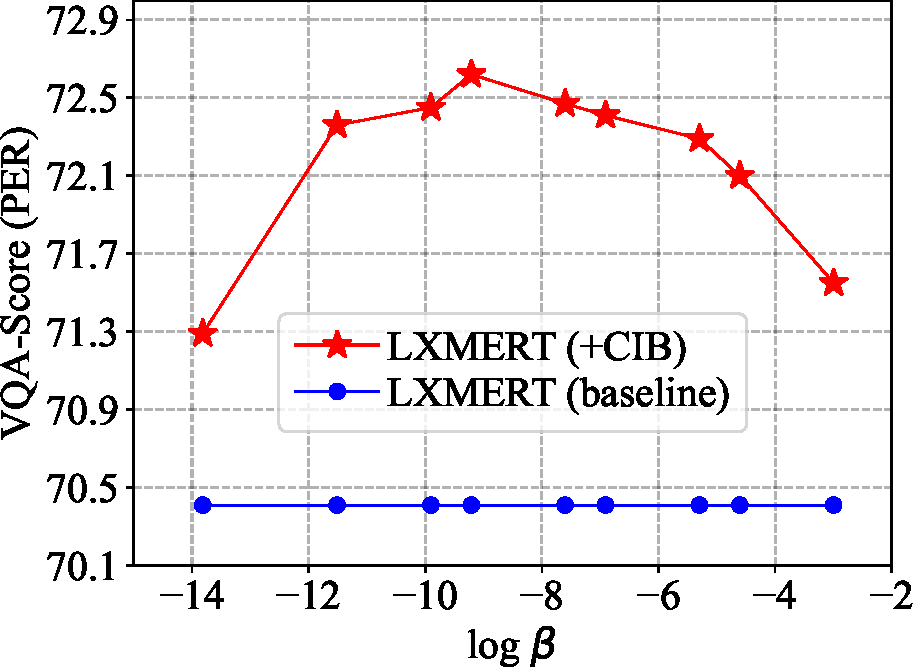
\includegraphics[height=3.7cm]{figure/c4_vis_lxmert_beta.pdf}
\subcaption{LXMERT}
\label{fig:c4_ph_2}
\end{subfigure}
\begin{subfigure}[b]{0.32\linewidth}
\centering
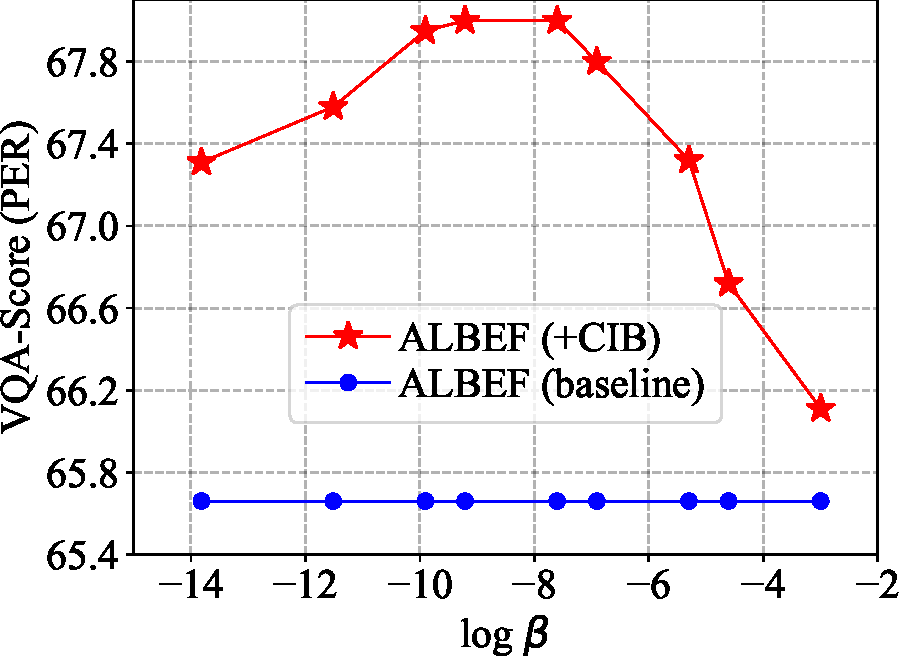
\includegraphics[height=3.7cm]{figure/c4_vis_albef_beta.pdf}
\subcaption{ALBEF}
\label{fig:c4_ph_3}
\end{subfigure}
\caption{在VQA-Rep上随$\log\beta$增加VQA-Score (\%)的变化曲线
}
\label{fig:c4_hp_beta}
\end{figure}
% ********************************************************************



\subsubsection{CIB不同上界的比较}
为了分析CIB中不同组成部分对视觉问答模型鲁棒性的贡献,本章对公式~(\ref{eq:c4_JMI})中不同项有意义的组合进行了消融实验。
具体来说,除了本章为CIB中多模态输入和表征间互信息推导的上界外,公式~(\ref{eq:c4_JMI})中的项还可以组成三种可证明的上界:
(\emph{i}) $\frac{3}{2}$ $[I(\Xmat^v; \Tmat^v) + I(\Xmat^l; \Tmat^l)]$ (即 \ding{202} + \ding{203});
(\emph{ii}) $-I(\Tmat^v; \Tmat^l) + \SKL$ (即 \ding{204} + \ding{205}) 和
(\emph{iii}) $I(\Xmat^v; \Tmat^v) + I(\Xmat^l; \Tmat^l) + \SKL$ (即 \ding{202} + \ding{203} + \ding{205})。
表~\ref{tab:c4_comp_ibs}比较了采用不同上界时CIB的性能,结果一致表明与其他形式的组合相比,本章节提出的CIB是$I(\Xmat^v, \Xmat^l; \Tmat^v, \Tmat^l)$更紧凑的上界。


\begin{table}[!t]
\caption{双流视觉语言模型不同中间表征对CIB的影响}
\label{tab:c4_lxmert_var}
\setlength{\tabcolsep}{16.mm}{
\begin{tabularx}{\linewidth}{@{}llc@{}}
\toprule 
VLMs
&\multicolumn{1}{c}{$\mathcal{L}_{\text{CIB}}$}
&VQA-Score (PER)
\\ 

\midrule[1pt]

\multirow{3}{*}{\makecell[l]{LXMERT~\citep{tan2019lxmert}}}
&$I(\Ymat; \Tmat)$
&70.41 
\\
&$I(\Ymat; \Tmat) - \beta I(\Xmat^v, \Xmat^l; \Tmat^{'v}, \Tmat^{'l})$
&72.53
\\
&$I(\Ymat; \Tmat) - \beta I(\Xmat^v, \Xmat^l; \Tmat^v, \Tmat^l)$ 
&\textbf{72.62} 
\\ 
\midrule
\multirow{3}{*}{\makecell[l]{ViLBERT~\cite{lu2019vilbert}}}
&$I(\Ymat; \Tmat)$
&59.16 
\\
&$I(\Ymat; \Tmat) - \beta I(\Xmat^v, \Xmat^l; \Tmat^{'v}, \Tmat^{'l})$
&62.23
\\
&$I(\Ymat; \Tmat) - \beta I(\Xmat^v, \Xmat^l; \Tmat^v, \Tmat^l)$ 
&\textbf{62.28} 
\\ 

\bottomrule
\end{tabularx}
}
\end{table}
\begin{table}[!t]
\caption{在VQA v2 test-dev上的实验结果 
% $^{\dagger}$表示该结果是我们对基线视觉语言预训练模型重新实现的结果。
}
\label{tab:c4_comp_vqa_v2_all} 
\setlength{\tabcolsep}{18.9mm}{
\begin{tabularx}{\linewidth}{@{}lrr}
\toprule
\multirow{2}{*}{VLMs} 
&\multicolumn{2}{c}{VQA-Score}
\\
\cmidrule(l){2-3}
&Baseline &+ CIB  
\\ 
\midrule[1pt] 
VisualBERT~\citep{li2019visualbert} 
&70.80 (70.46\textcolor{red}{$^{\dagger}$}) 
&\cellcolor{gray!15}71.62 \positive{\uparrow 1.16}
\\ 

VL-T5~\citep{cho2021unifying}
&- (70.23\textcolor{red}{$^{\dagger}$}) 
&71.14\cellcolor{gray!15} \positive{\uparrow 0.91} 
\\

LXMERT~\citep{tan2019lxmert} 
&72.42 (72.58\textcolor{red}{$^{\dagger}$})
&\cellcolor{gray!15}72.99 \positive{\uparrow 0.41}
\\ 

UNITER$_{\text{B}}$~\citep{chen2020uniter} 
&72.70 (71.63\textcolor{red}{$^{\dagger}$})
&\cellcolor{gray!15}72.11 \positive{\uparrow 0.48} 
\\ 

ALBEF~\citep{li2021align}
&74.54 (74.54\textcolor{red}{$^{\dagger}$}) 
&76.27\cellcolor{gray!15} \positive{\uparrow 1.73} 
\\

ViLBERT~\citep{lu2019vilbert} 
&70.55 (70.55\textcolor{red}{$^{\dagger}$}) 
&\cellcolor{gray!15}71.00 \positive{\uparrow 0.45}
\\ 

VL-BERT$_{\text{B}}$~\citep{su2019vl} 
&71.16 (71.20\textcolor{red}{$^{\dagger}$}) 
&\cellcolor{gray!15}71.59 \positive{\uparrow 0.39} 
\\ 

\bottomrule 
\end{tabularx}
}
\end{table}


\subsubsection{不同互信息估计器的影响}
事实上,任何基于采样的互信息上界估计器都可用于逼近$I(\Xmat^v; \Tmat^v)$ 和 $I(\Xmat^l; \Tmat^l)$。
任何可微的互信息下界估计器都可用于逼近$I(\Tmat^v; \Tmat^l)$。
为了分析不同互信息估计器的影响,本章考虑以下实验设置:
(\emph{i}) 使用L1Out~\cite{poole2019variational}替代CLUB~\cite{cheng2020club}作为互信息上界估计器逼近$I(\Xmat^v; \Tmat^v)$ 和 $I(\Xmat^l; \Tmat^l)$;
(\emph{ii}) 分别使用互信息下界估计器InfoNCE~\cite{oord2018representation}、 NWJ~\cite{nguyen2010estimating}和 MINE~\cite{belghazi2018mine}逼近$I(\Tmat^v; \Tmat^l)$。
表~\ref{tab:c4_comp_ibs}中的实验结果表明CIB在提高视觉问答模型输入鲁棒性方面的有效性并不明显依赖于特定的互信息估计器。



\subsubsection{超参数的影响}
公式~(\ref{eq:CIB})中的超参$\beta$控制着表征冗余和压缩之间的平衡,是CIB中的核心超参数。
因此,本章对$\beta$进行网格搜索。
具体来说,本章考虑以下$\beta$值,即,$\beta \in [1\times10^{-6}, 1\times10^{-5}, 5\times10^{-5}, 1\times10^{-4}, 5\times10^{-4}, 1\times10^{-3}, 5\times10^{-3}, 1\times10^{-2}, 5\times10^{-2}]$。
图~\ref{fig:c4_hp_beta} 展示了在VQA-Rep数据集上VQA-Score (PER)的变化曲线。本章发现VQA-Score在$\beta$取很小值时就开始增加(这表明了CIB的有效性)。
当$\beta$增加到$5\times10^{-5}$、$1\times10^{-4}$ 和 $1\times10^{-4}$时,以UNITER$_\text{B}$、LXMERT和ALBEF为基线的视觉问答模型分别取得了最好的性能。
随后,VQA-Score开始下降,这表明对视觉语言预训练模型表征过度的压缩反而会损害视觉问答模型的鲁棒性。






% ********************************************************************
\begin{figure}[!t]
\centering
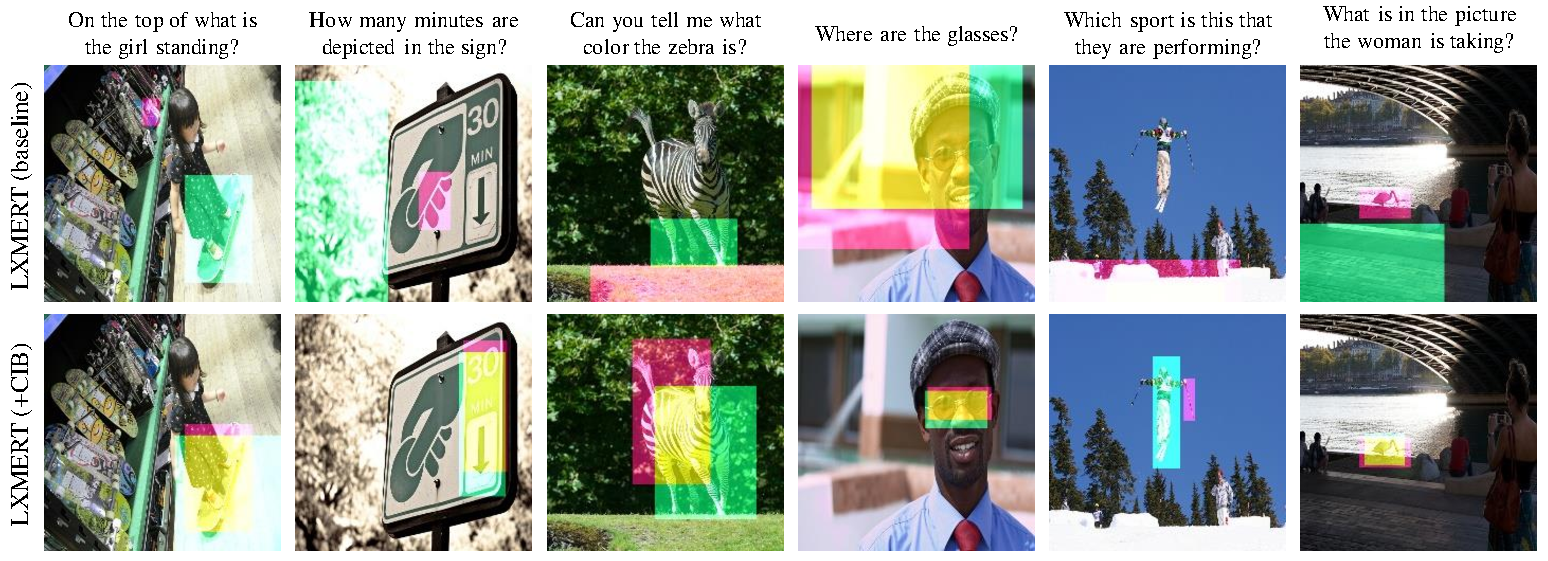
\includegraphics[width=1.0\linewidth]{figure/c4_hm.pdf}
\caption{在VQA-Rep数据集上注意力得分最高的两个物体的可视化}
\label{fig:c4_example_hm}
\end{figure}
% ********************************************************************

% ***************************************************************** 
\begin{figure*}[!t] 
\begin{subfigure}[b]{1.0\textwidth}
\centering
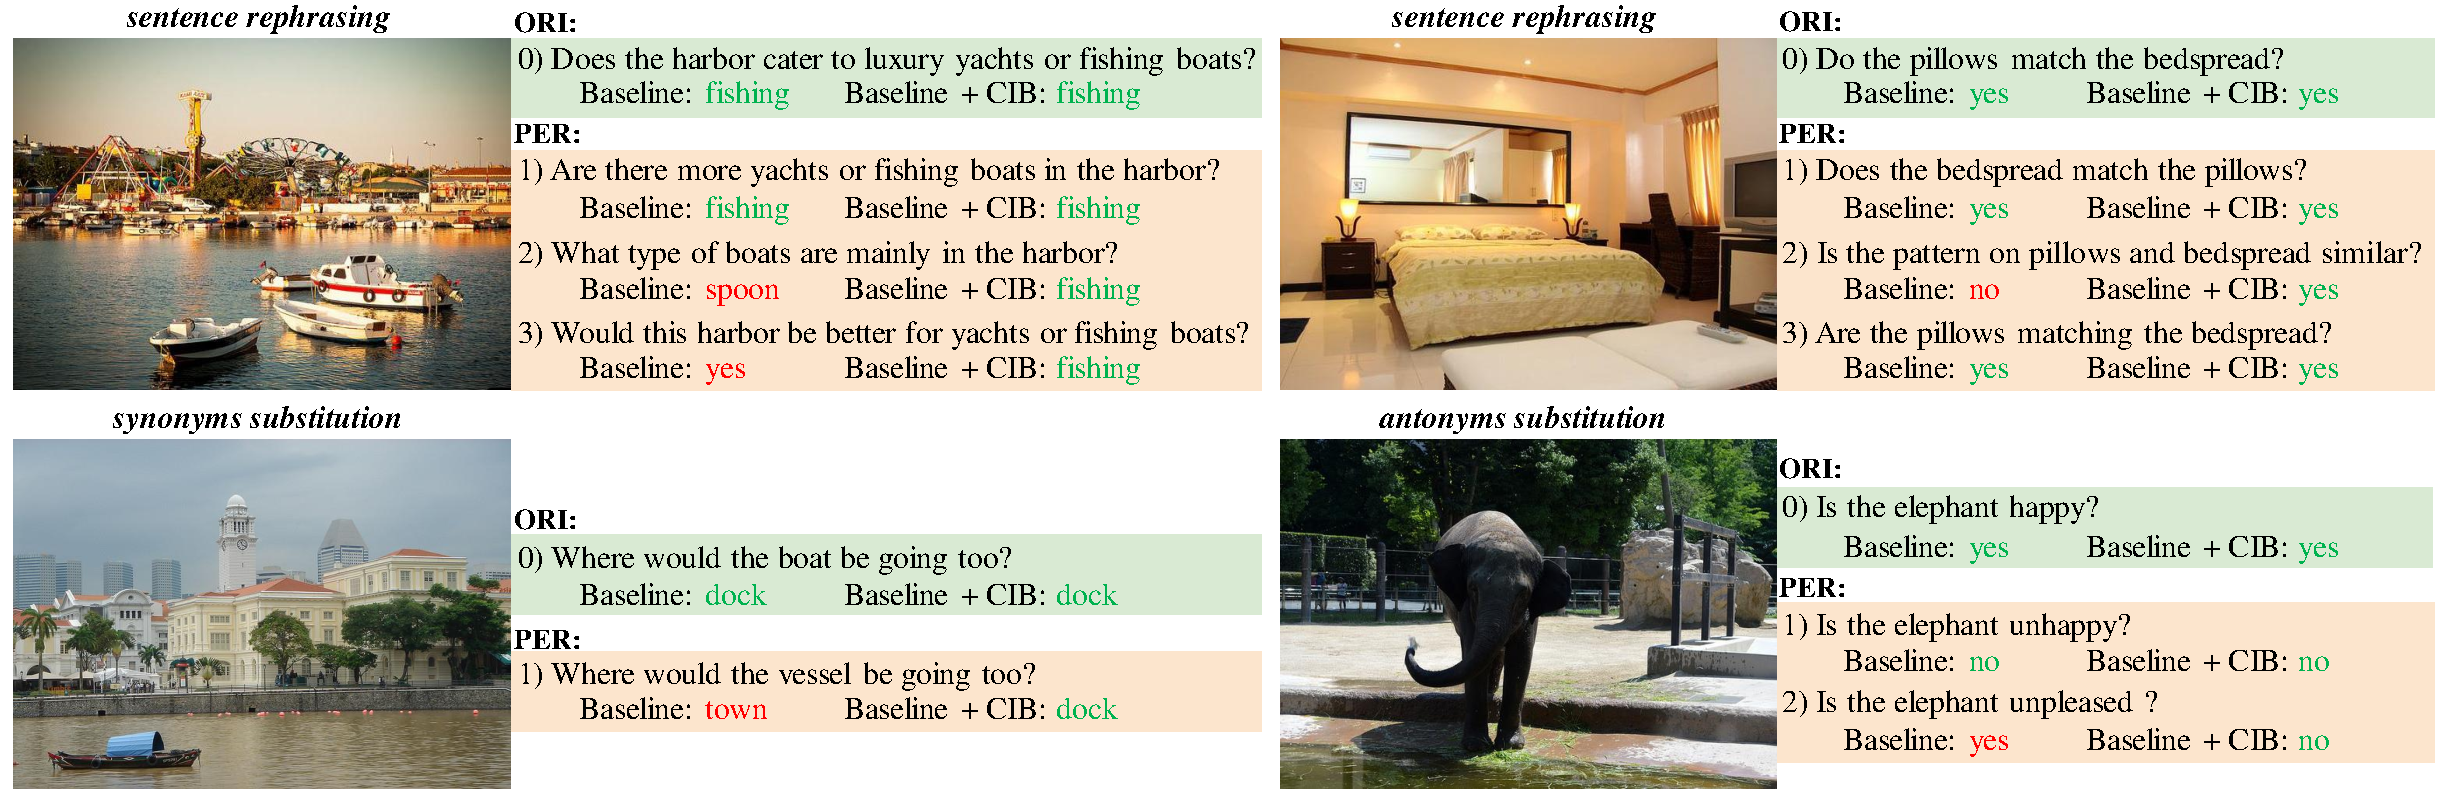
\includegraphics[width=0.99\linewidth]{figure/c4_vis_rlv1.pdf}
\subcaption{对语言输入变化的鲁棒性举例}
\label{fig:vis_lv}
\end{subfigure}
\begin{subfigure}[b]{\linewidth}
\includegraphics[width=0.99\linewidth]{figure/c4_vis_rvv1.pdf}
\subcaption{对视觉输入变化的鲁棒性举例}
\label{fig:vis_vv}
\end{subfigure}
\begin{subfigure}[b]{\linewidth}
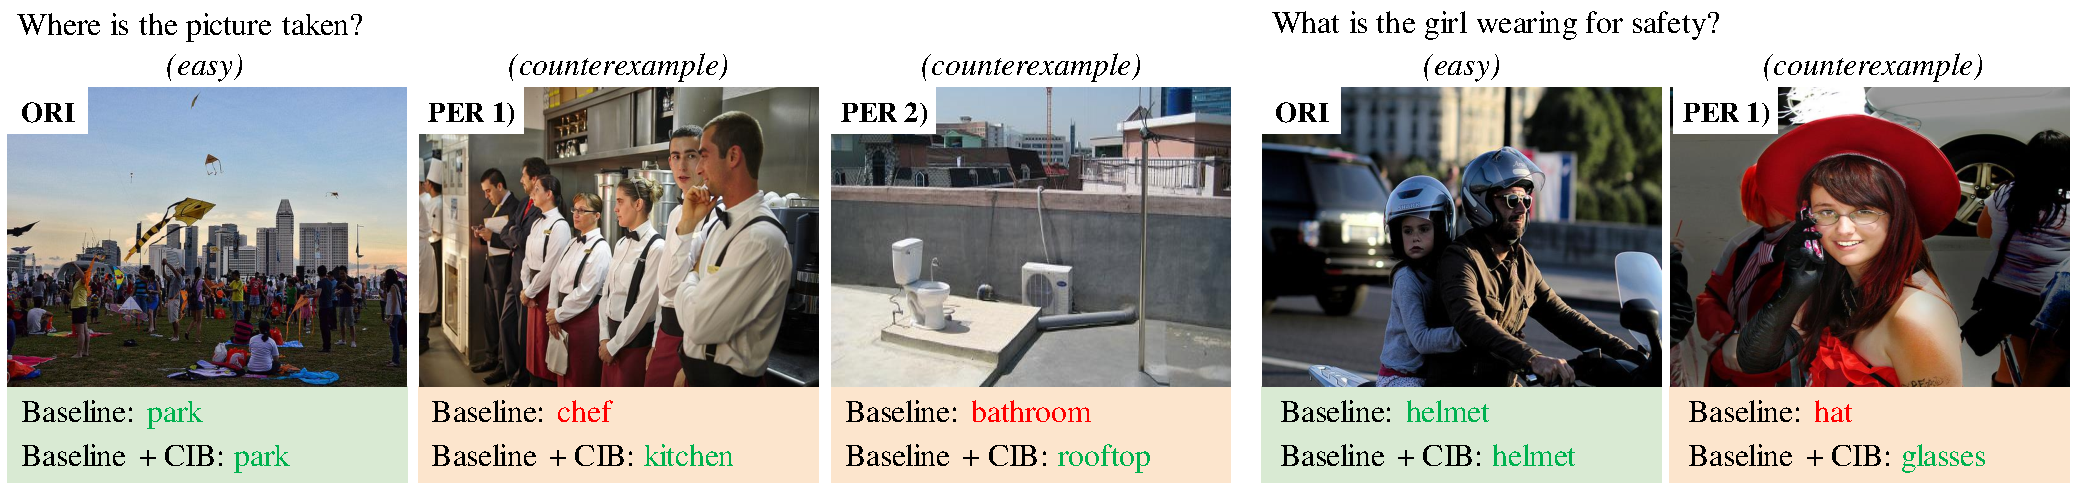
\includegraphics[width=0.99\linewidth]{figure/c4_vis_rscl1.pdf}
\subcaption{对捷径学习的鲁棒性举例}
\label{fig:vis_sc}
\end{subfigure}
\vspace{-6mm}
\caption{定性实验结果对比}
\label{fig:vis_example}
\vspace{-4mm}
\end{figure*}
% ********************************************************************


% **************************************************************************
\subsubsection{视觉语言模型不同的中间表征对CIB的影响}
如图~\ref{fig:c4_cib} 所示,对于具有双流编码器(LXMERT 和 ViLBERT)的预训练视觉语言模型,还存在另一种中间表征方法,即通过视觉Transformer 层($f_{\theta^{\text{VTran}}}$)和 语言Transformer 层($f_{\theta^{\text{LTran}}}$)后得到的视觉和语言表征 $\Tmat=[\Tmat^{'v}, \Tmat^{'l}]$。
当使用 CIB 对双流预训练视觉语言模型进行微调时,为了分析不同中间表征的影响,本章将 $\mathcal{L}_{\text{CIB}}$ 中的原始 $\Tmat=[\Tmat^{'v}, \Tmat^{'l}]$ 替换为 $\Tmat=[\Tmat^{'v}, \Tmat^{'l}]$。
从表~\ref{tab:c4_lxmert_var} 的结果中,本章发现不同的中间表征对 CIB 的性能影响较小,这表明对于具有双流预训练视觉语言模型的模型,使用视觉和语言 Transformer 层之后的视觉和语言表征作为中间表征来估计 $\mathcal{L}_{\text{CIB}}$ 中的互信息项也是可行的。



\begin{table}[!t]
\caption{RefCOCO+~\citep{yu2016modeling}数据集上弱监督视觉定位的实验结果
}
\label{tab:c4_vg}
\setlength{\tabcolsep}{18.35mm}{
\begin{tabularx}{\linewidth}{@{}lccc@{}}
\toprule
Method &Val &TestA &TestB
\\
% \cmidrule(l){2-4}
\midrule[1pt]
ARN~\citep{liu2019adaptive} 
&32.78 &34.35 &32.13
\\
CCL~\citep{zhang2020counterfactual}
&34.29 &36.91 &33.56
\\
ALBEF$_{\text{itc}}$~\citep{li2021align}
&51.58 &60.09 &40.19
\\
ALBEF$_{\text{itm}}$~\citep{li2021align}
&58.46 &65.89 &46.25
\\
\quad + Our CIB
&\textbf{59.41} &\textbf{67.39} &\textbf{47.18}
\\
\bottomrule 
\end{tabularx}
}
\end{table}


% **************************************************************************
\subsubsection{CIB对标准视觉问答性能的影响}

为了分析在标准视觉问答数据集上评测时CIB是否会对视觉问答模型的性能产生影响,本章使用CIB作为训练目标在VQA v2的训练集和验证集上微调上述七种基线视觉语言预训练模型。
在VQA v2 测试集上的实验结果如表~\ref{tab:c4_comp_vqa_v2_all}所示。
\textcolor{red}{$^{\dagger}$}表示该结果是本章对基线视觉语言预训练模型重新实现的结果。
整体来说,使用本章提出的CIB训练基线视觉语言预训练模型也能小幅度地提高视觉问答模型在标准视觉问答数据集VQA v2上性能。
由此,本章发现对表征进行一定程度的压缩可以使得到的表征更加紧凑和鲁棒,有利于视觉语言预训练模型学习表征和标签之间更真实的相关。



% **************************************************************************
\subsubsection{CIB在其它多模态任务上的泛化能力}
为了验证CIB在其它多模态任务上的有效性,本章考虑了弱监督视觉定位任务。
遵循Li等人~\cite{li2021align} 原始的实验设定,在RefCOCO+~\cite{yu2016modeling}训练集上使用本章所提的CIB微调预训练的ALBEF。
从表\ref{tab:c4_vg}中的实验结果可以发现,使用CIB可以进一步提高基线ALBEF$_{\text{itm}}$的性能,表明所提出的CIB可以有效地应用于其它多模态任务。




% **************************************************************************
\xsubsection{定性实验}{Qualitative Experiment}



\subsubsection{CIB提高基线预训练视觉语言模型的输入鲁棒性的解释}

本章以LXMERT~\cite{tan2019lxmert}作为基线预训练视觉语言模型的代表并进行以下实验来研究可能的原因。
具体来说,本章首先列举了在VQA-Rep数据集中,使用CIB 微调后的LXMERT能够正确预测答案但基线LXMERT无法正确预测答案的图像-问题对。
然后,本章通过公式$\text{score}_\text{attn} = \softmax(\Zmat \cdot (\Xmat^{v})^{\mathsf{T}}/\sqrt{d})$计算了用于答案预测的最终表征$\Zmat \in \mathbb{R}^d$与目标区域的输入视觉特征$\Xmat^v \in \mathbb{R}^{K\times d}$之间的注意力分数。
最后,本章使用\textcolor{magenta}{洋红色}和\textcolor{green}{绿色}来突出显示图像中具有最高注意力分数的前两个物体。
从图~\ref{fig:c4_example_hm} 的结果中,本章观察到相对于基准 LXMERT,通过 CIB 微调后的 LXMERT 得到的注意力机制关注的两个对象更加一致和与问题相关。
这一观察定性地说明,将 CIB 作为训练目标用于 微调 预训练视觉语言模型可以鼓励模型学习更具有区分性的表征,以应对不同的答案,并减少与问题无关的信息。


\subsubsection{定性实验结果}
图~\ref{fig:vis_lv}、\ref{fig:vis_vv}和\ref{fig:vis_sc} 分别展示了对输入语言变化、视觉变化和多模态捷径学习的鲁棒性的举例。
根据图中的定性对比,本章可以观察到相对于使用交叉熵损失微调预训练 LXMERT 的基线,使用本章提出的CIB 作为训练目标微调预训练视觉语言模型可以提高视觉问答模型正确回答这些有挑战的问题的能力,这从经验上证明了 CIB 在防御此类涉及视觉和语言输入变化的攻击方面的有效性。




% **************************************************************************
\xsection{本章小结}{Summary}

本章提出了一种基于相关信息瓶颈理论的鲁棒视觉问答方法。
该方法以相关信息瓶颈理论为训练目标,在将视觉语言预训练模型迁移到视觉问答任务时,通过最小化输入与表征之间的相互信息并最大化输出和表征之间的互信息来平衡表征中的信息压缩和冗余,有效地提高了模型的输入鲁棒性。
此外,为了更准确地估计多模态输入和表征之间的互信息,本章推导了兼顾不同模态输入和表征之间的内部关联的紧凑互信息上界,以此来指导视觉问答模型学习更鲁棒的表征并促进多模态对齐。
在五个输入鲁棒性的视觉问答数据集上进行的广泛实验一致证明了CIB的鲁棒性和性能优越性。
在未来,我们的目标是探索一种新方法,以在将视觉语言预训练模型迁移到小样本场景时能更好地提高模型的泛化能力。
